%package list
\documentclass{article}
\usepackage[top=3cm, bottom=3cm, outer=3cm, inner=3cm]{geometry}
\usepackage{multicol}
\usepackage{graphicx}
\usepackage{url}
%\usepackage{cite}
\usepackage{hyperref}
\usepackage{array}
%\usepackage{multicol}
\newcolumntype{x}[1]{>{\centering\arraybackslash\hspace{0pt}}p{#1}}
\usepackage{natbib}
\usepackage{pdfpages}
\usepackage{multirow}
\usepackage[normalem]{ulem}
\useunder{\uline}{\ul}{}
\usepackage{svg}
\usepackage{xcolor}
\usepackage{listings}
\lstdefinestyle{ascii-tree}{
    literate={├}{|}1 {─}{--}1 {└}{+}1 
  }
\lstset{basicstyle=\ttfamily,
  showstringspaces=false,
  commentstyle=\color{red},
  keywordstyle=\color{blue}
}
%\usepackage{booktabs}
\usepackage{caption}
\usepackage{subcaption}
\usepackage{float}
\usepackage{array}

\usepackage{enumitem}


\newcolumntype{M}[1]{>{\centering\arraybackslash}m{#1}}
\newcolumntype{N}{@{}m{0pt}@{}}


%%%%%%%%%%%%%%%%%%%%%%%%%%%%%%%%%%%%%%%%%%%%%%%%%%%%%%%%%%%%%%%%%%%%%%%%%%%%
%%%%%%%%%%%%%%%%%%%%%%%%%%%%%%%%%%%%%%%%%%%%%%%%%%%%%%%%%%%%%%%%%%%%%%%%%%%%
\newcommand{\itemEmail}{eportugalpor@unsa.edu.pe hchoquehuancaz@unsa.edu.pe}
\newcommand{\itemStudent}{Eduardo Portugal \& Hernan Choquehuanca}
\newcommand{\itemCourse}{Fundamentos de Programación 2}
\newcommand{\itemCourseCode}{1701213}
\newcommand{\itemSemester}{II}
\newcommand{\itemUniversity}{Universidad Nacional de San Agustín de Arequipa}
\newcommand{\itemFaculty}{Facultad de Ingeniería de Producción y Servicios}
\newcommand{\itemDepartment}{Departamento Académico de Ingeniería de Sistemas e Informática}
\newcommand{\itemSchool}{Escuela Profesional de Ingeniería de Sistemas}
\newcommand{\itemAcademic}{2023 - B}
\newcommand{\itemInput}{Del 22 Enero 2024}
\newcommand{\itemOutput}{Al 29 Enero 2024}
\newcommand{\itemPracticeNumber}{Final}
\newcommand{\itemTheme}{Proyecto Final - Videojuego}
%%%%%%%%%%%%%%%%%%%%%%%%%%%%%%%%%%%%%%%%%%%%%%%%%%%%%%%%%%%%%%%%%%%%%%%%%%%%
%%%%%%%%%%%%%%%%%%%%%%%%%%%%%%%%%%%%%%%%%%%%%%%%%%%%%%%%%%%%%%%%%%%%%%%%%%%%

\usepackage[english,spanish]{babel}
\usepackage[utf8]{inputenc}
\AtBeginDocument{\selectlanguage{spanish}}
\renewcommand{\figurename}{Figura}
\renewcommand{\refname}{Referencias}
\renewcommand{\tablename}{Tabla} %esto no funciona cuando se usa babel
\AtBeginDocument{%
	\renewcommand\tablename{Tabla}
}

\usepackage{fancyhdr}
\pagestyle{fancy}
\fancyhf{}
\setlength{\headheight}{30pt}
\renewcommand{\headrulewidth}{1pt}
\renewcommand{\footrulewidth}{1pt}
\fancyhead[L]{\raisebox{-0.2\height}{
\includegraphics[width=3cm]{img/logo_episunsa.png}}}
\fancyhead[C]{\fontsize{7}{7}\selectfont	\itemUniversity \\ \itemFaculty \\ \itemDepartment \\ \itemSchool \\ \textbf{\itemCourse}}
\fancyhead[R]{\raisebox{-0.2\height}{
\includegraphics[width=1.2cm]{img/logo_abet}}}
\fancyfoot[L]{Eduardo P. P., Hernan C. Z.}
\fancyfoot[C]{\itemCourse}
\fancyfoot[R]{Página \thepage}

% para el codigo fuente
\usepackage{listings}
\usepackage{color, colortbl}
\definecolor{dkgreen}{rgb}{0,0.6,0}
\definecolor{gray}{rgb}{0.5,0.5,0.5}
\definecolor{mauve}{rgb}{0.58,0,0.82}
\definecolor{codebackground}{rgb}{0.95, 0.95, 0.92}
\definecolor{tablebackground}{rgb}{0.8, 0, 0}

\lstset{frame=tb,
	language=bash,
	aboveskip=3mm,
	belowskip=3mm,
	showstringspaces=false,
	columns=flexible,
	basicstyle={\small\ttfamily},
	numbers=none,
	numberstyle=\tiny\color{gray},
	keywordstyle=\color{blue},
	commentstyle=\color{dkgreen},
	stringstyle=\color{mauve},
	breaklines=true,
	breakatwhitespace=true,
	tabsize=3,
	backgroundcolor= \color{codebackground},
}

\begin{document}
	
	\vspace*{10px}
	
	\begin{center}	
		\fontsize{17}{17} \textbf{ Informe de Laboratorio \itemPracticeNumber}
	\end{center}
	\centerline{\textbf{\Large Tema: \itemTheme}}
	%\vspace*{0.5cm}	

	\begin{flushright}
		\begin{tabular}{|M{2.5cm}|N|}
			\hline 
			\rowcolor{tablebackground}
			\color{white} \textbf{Nota}  \\
			\hline 
			     \\[30pt]
			\hline 			
		\end{tabular}
	\end{flushright}	

	\begin{table}[H]
		\begin{tabular}{|x{4.7cm}|x{4.8cm}|x{4.8cm}|}
			\hline 
			\rowcolor{tablebackground}
			\color{white} \textbf{Estudiante} & \color{white}\textbf{Escuela}  & \color{white}\textbf{Asignatura}   \\
			\hline 
			{\itemStudent \par \itemEmail} & \itemSchool & {\itemCourse \par Semestre: \itemSemester \par Código: \itemCourseCode}     \\
			\hline 			
		\end{tabular}
	\end{table}		
	
	\begin{table}[H]
		\begin{tabular}{|x{4.7cm}|x{4.8cm}|x{4.8cm}|}
			\hline 
			\rowcolor{tablebackground}
			\color{white}\textbf{Laboratorio} & \color{white}\textbf{Tema}  & \color{white}\textbf{Duración}   \\
			\hline 
			\itemPracticeNumber & \itemTheme & 72 horas   \\
			\hline 
		\end{tabular}
	\end{table}
	
	\begin{table}[H]
		\begin{tabular}{|x{4.7cm}|x{4.8cm}|x{4.8cm}|}
			\hline 
			\rowcolor{tablebackground}
			\color{white}\textbf{Semestre académico} & \color{white}\textbf{Fecha de inicio}  & \color{white}\textbf{Fecha de entrega}   \\
			\hline 
			\itemAcademic & \itemInput &  \itemOutput  \\
			\hline 
		\end{tabular}
	\end{table}
	
	\section{Tarea}
	\begin{itemize}		
		\item Terminar trabajo final - VideoJuego
	\end{itemize}
		
	\section{Equipos, materiales y temas utilizados}
	\begin{itemize}
		\item Sistema Operativo Windows 11 Home Single Language 22H2 64 bits.
		\item Visual Studio Code 1.82.2.0.
		\item JDK 17 Full 64-Bits 17.0.7.7.
		\item Git 2.41.0.2.
		\item Cuenta en GitHub con el correo institucional.
	\end{itemize}
	
	\section{URL de Repositorio Github}
	\begin{itemize}
		\item URL del Repositorio GitHub para clonar o recuperar.
		\item \url{https://github.com/hernanchoquehuanca/fp2-23b.git}
		\item URL para el laboratorio final en el Repositorio GitHub.
		\item \url{https://github.com/hernanchoquehuanca/fp2-23b/tree/main/fase03/proyecto_final}
	\end{itemize}
	
	\section{Laboratorio Final}
	
	\begin{itemize}	
		\item A continuación se mostrara el desarrollo del ejercicio de laboratorio:
	\end{itemize}
	
	\subsection{Diagrama UML de clases}
	
	\begin{figure}[H]
        \centering
		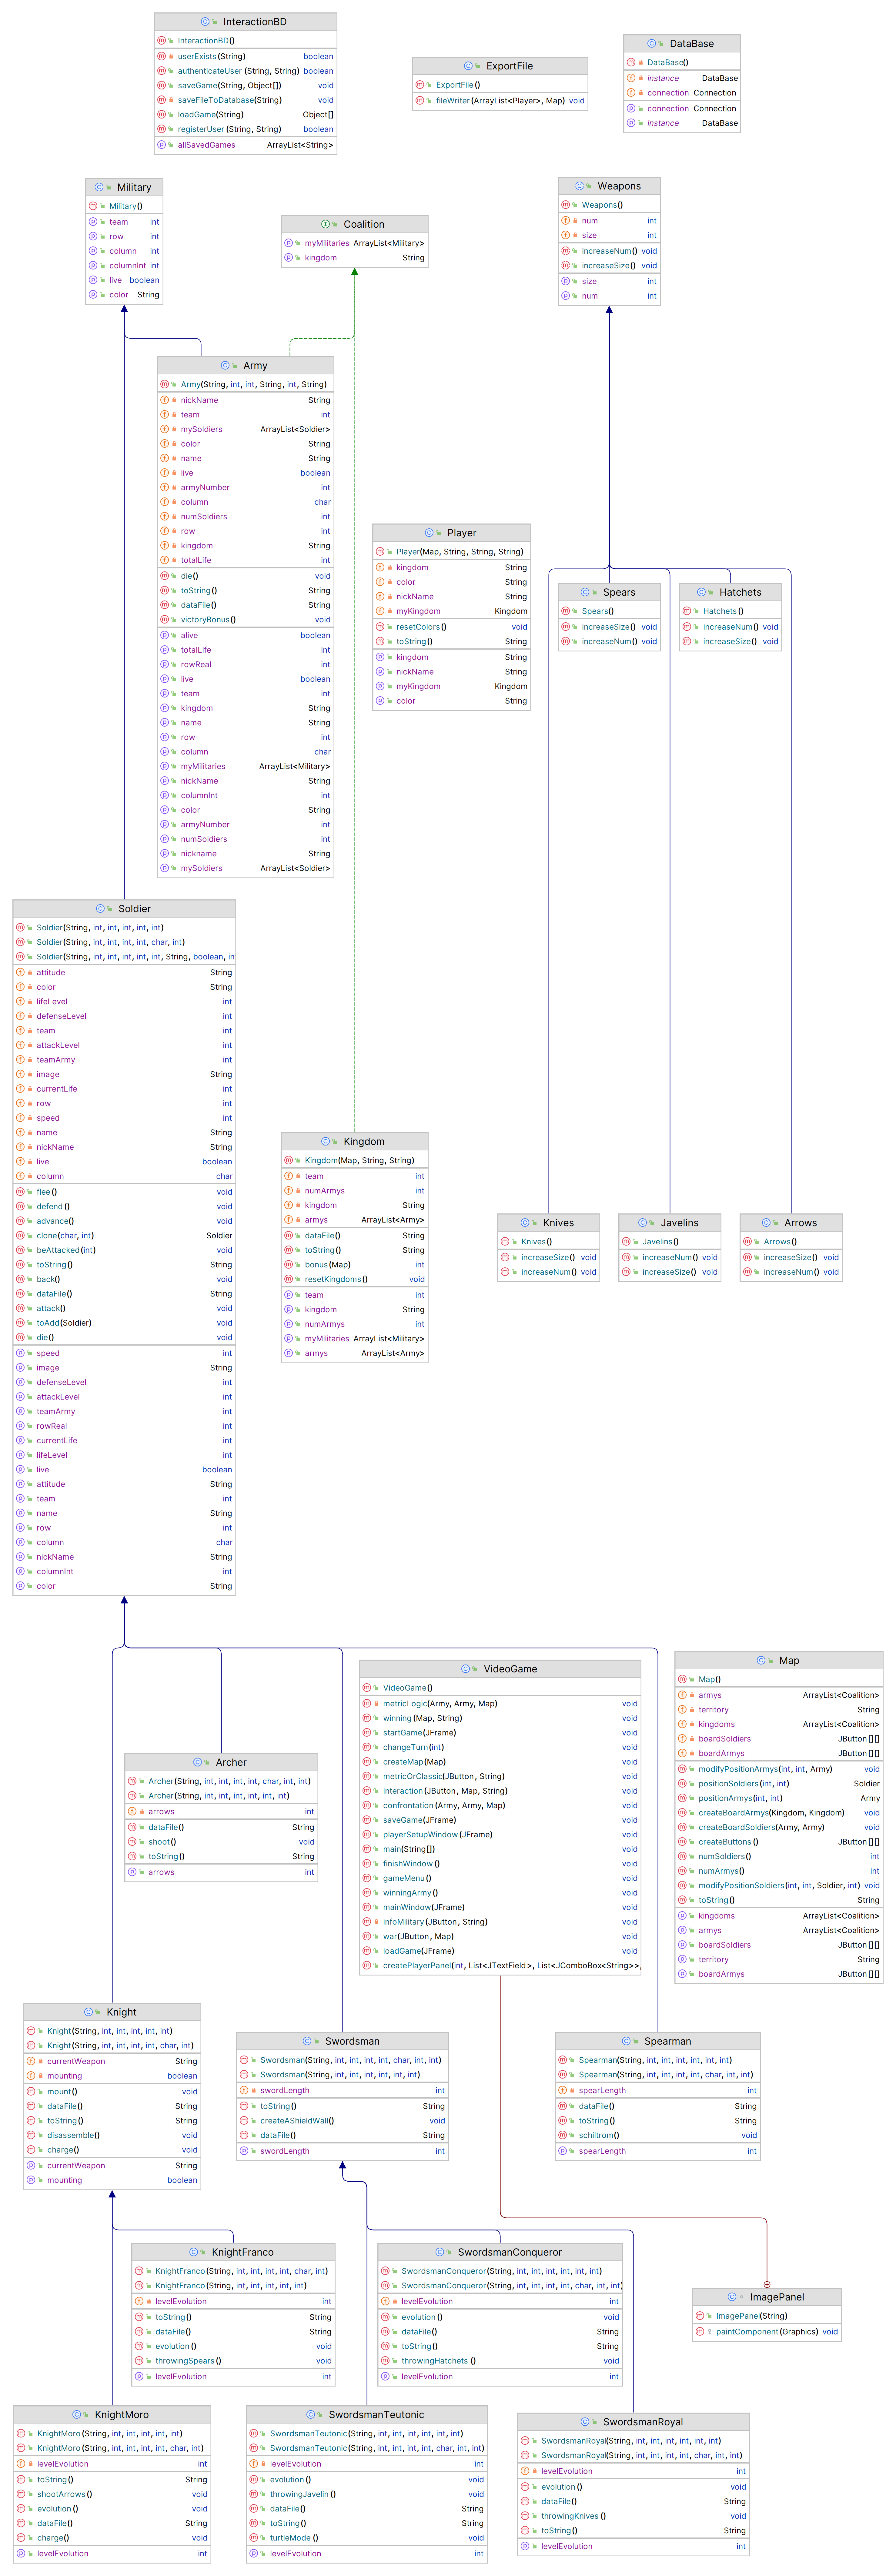
\includegraphics[width=0.4\textwidth,keepaspectratio]{img/DiagramaUML.png}
        \caption{Click \href{https://github.com/hernanchoquehuanca/fp2-23b/blob/main/fase03/proyecto_final/latex/img/DiagramaUML.png}{aquí} para ver Diagrama UML de clases completo - Demasiado Grande}
    \end{figure}
    
    \begin{figure}[H]
        \centering
		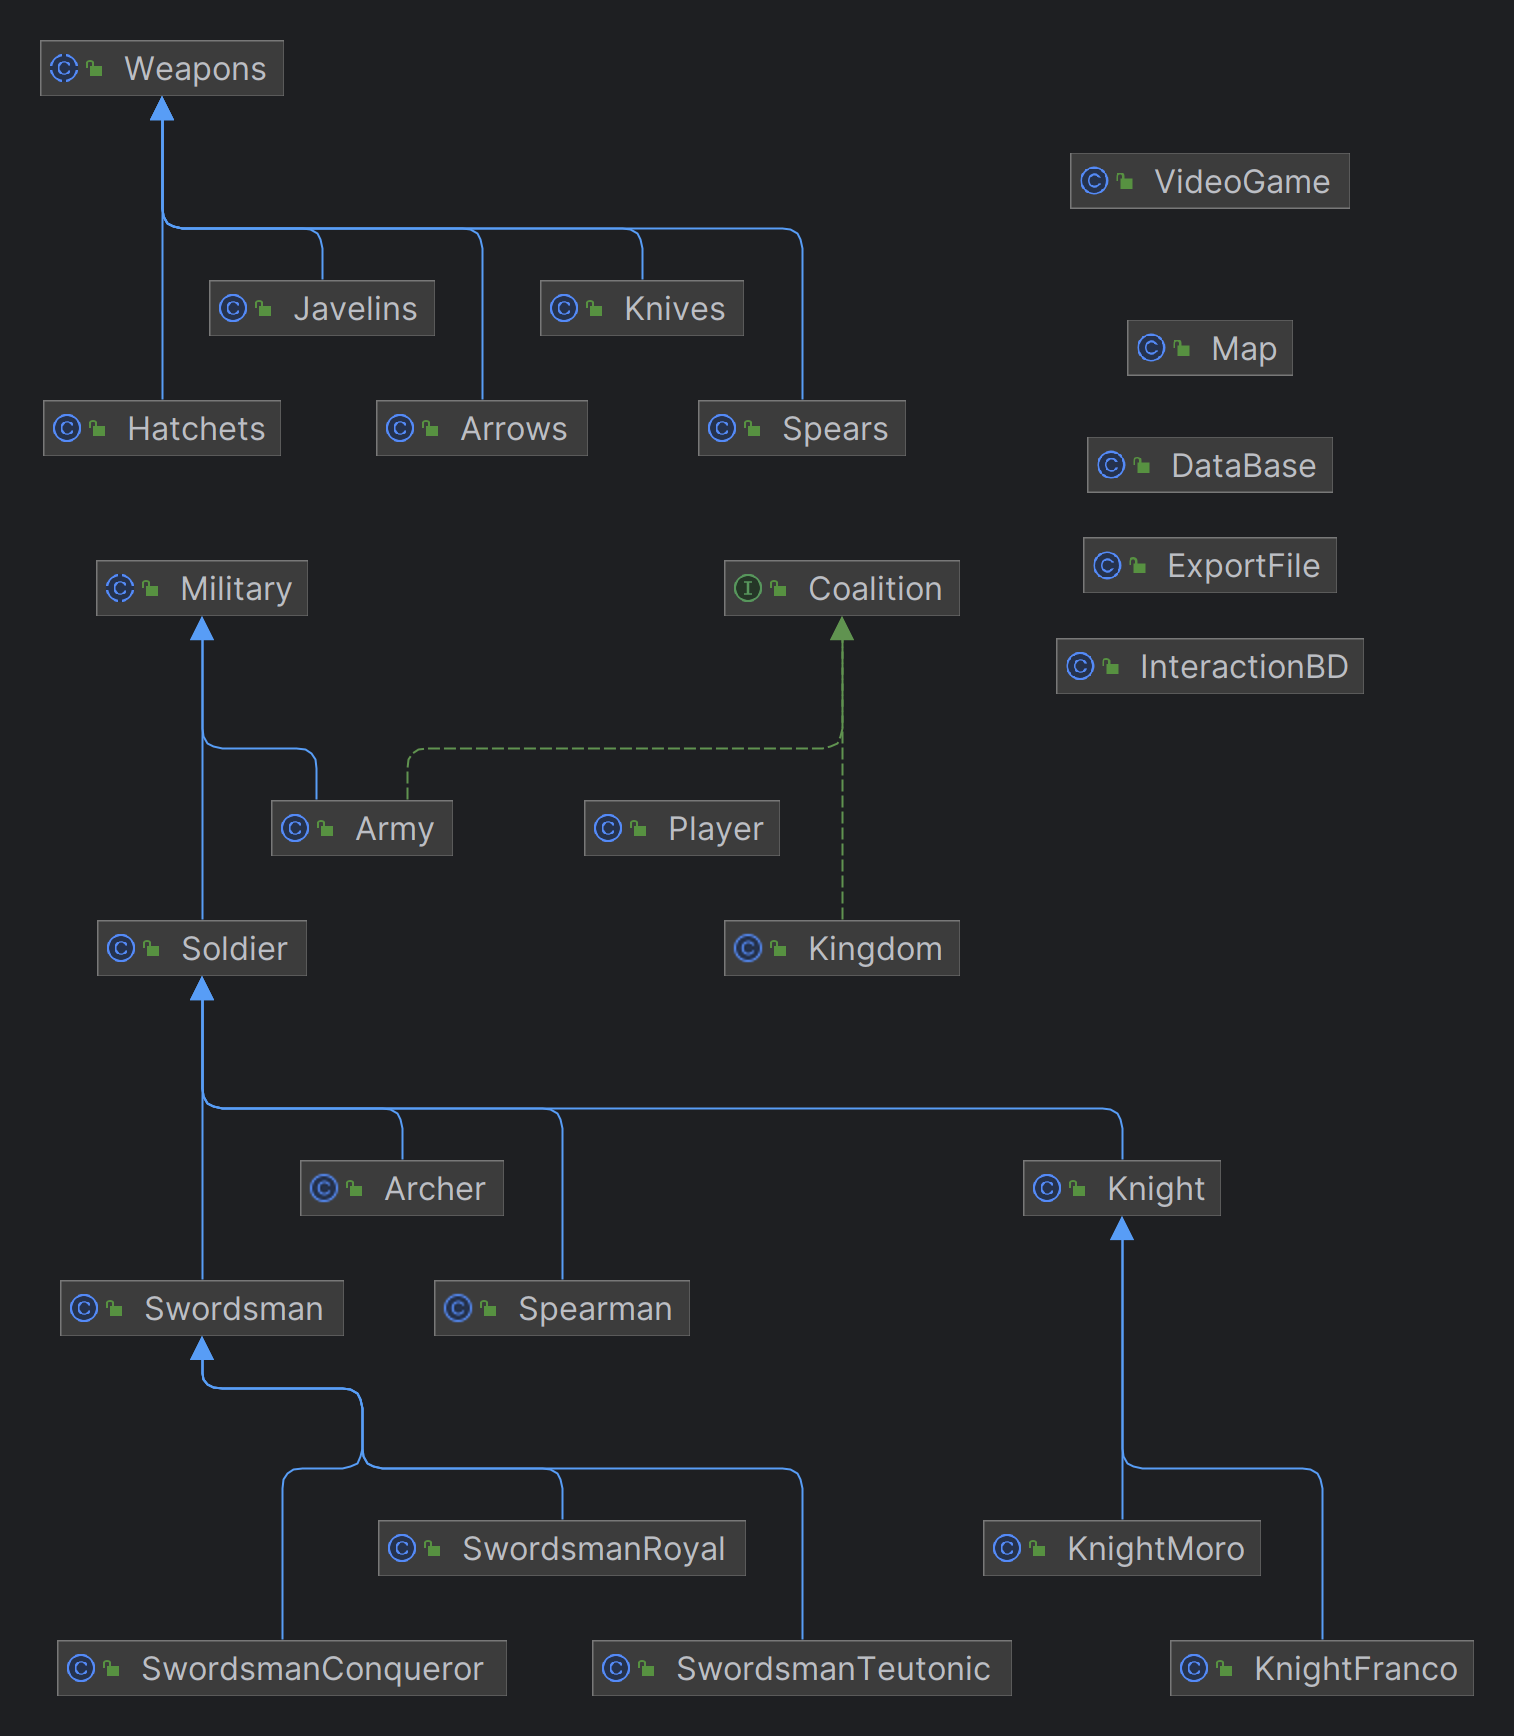
\includegraphics[width=0.9\textwidth,keepaspectratio]{img/DiagramaUML1.png}
        \caption{Relaciones de herencia entre las clases}
    \end{figure}
    
    \begin{figure}[H]
        \centering
		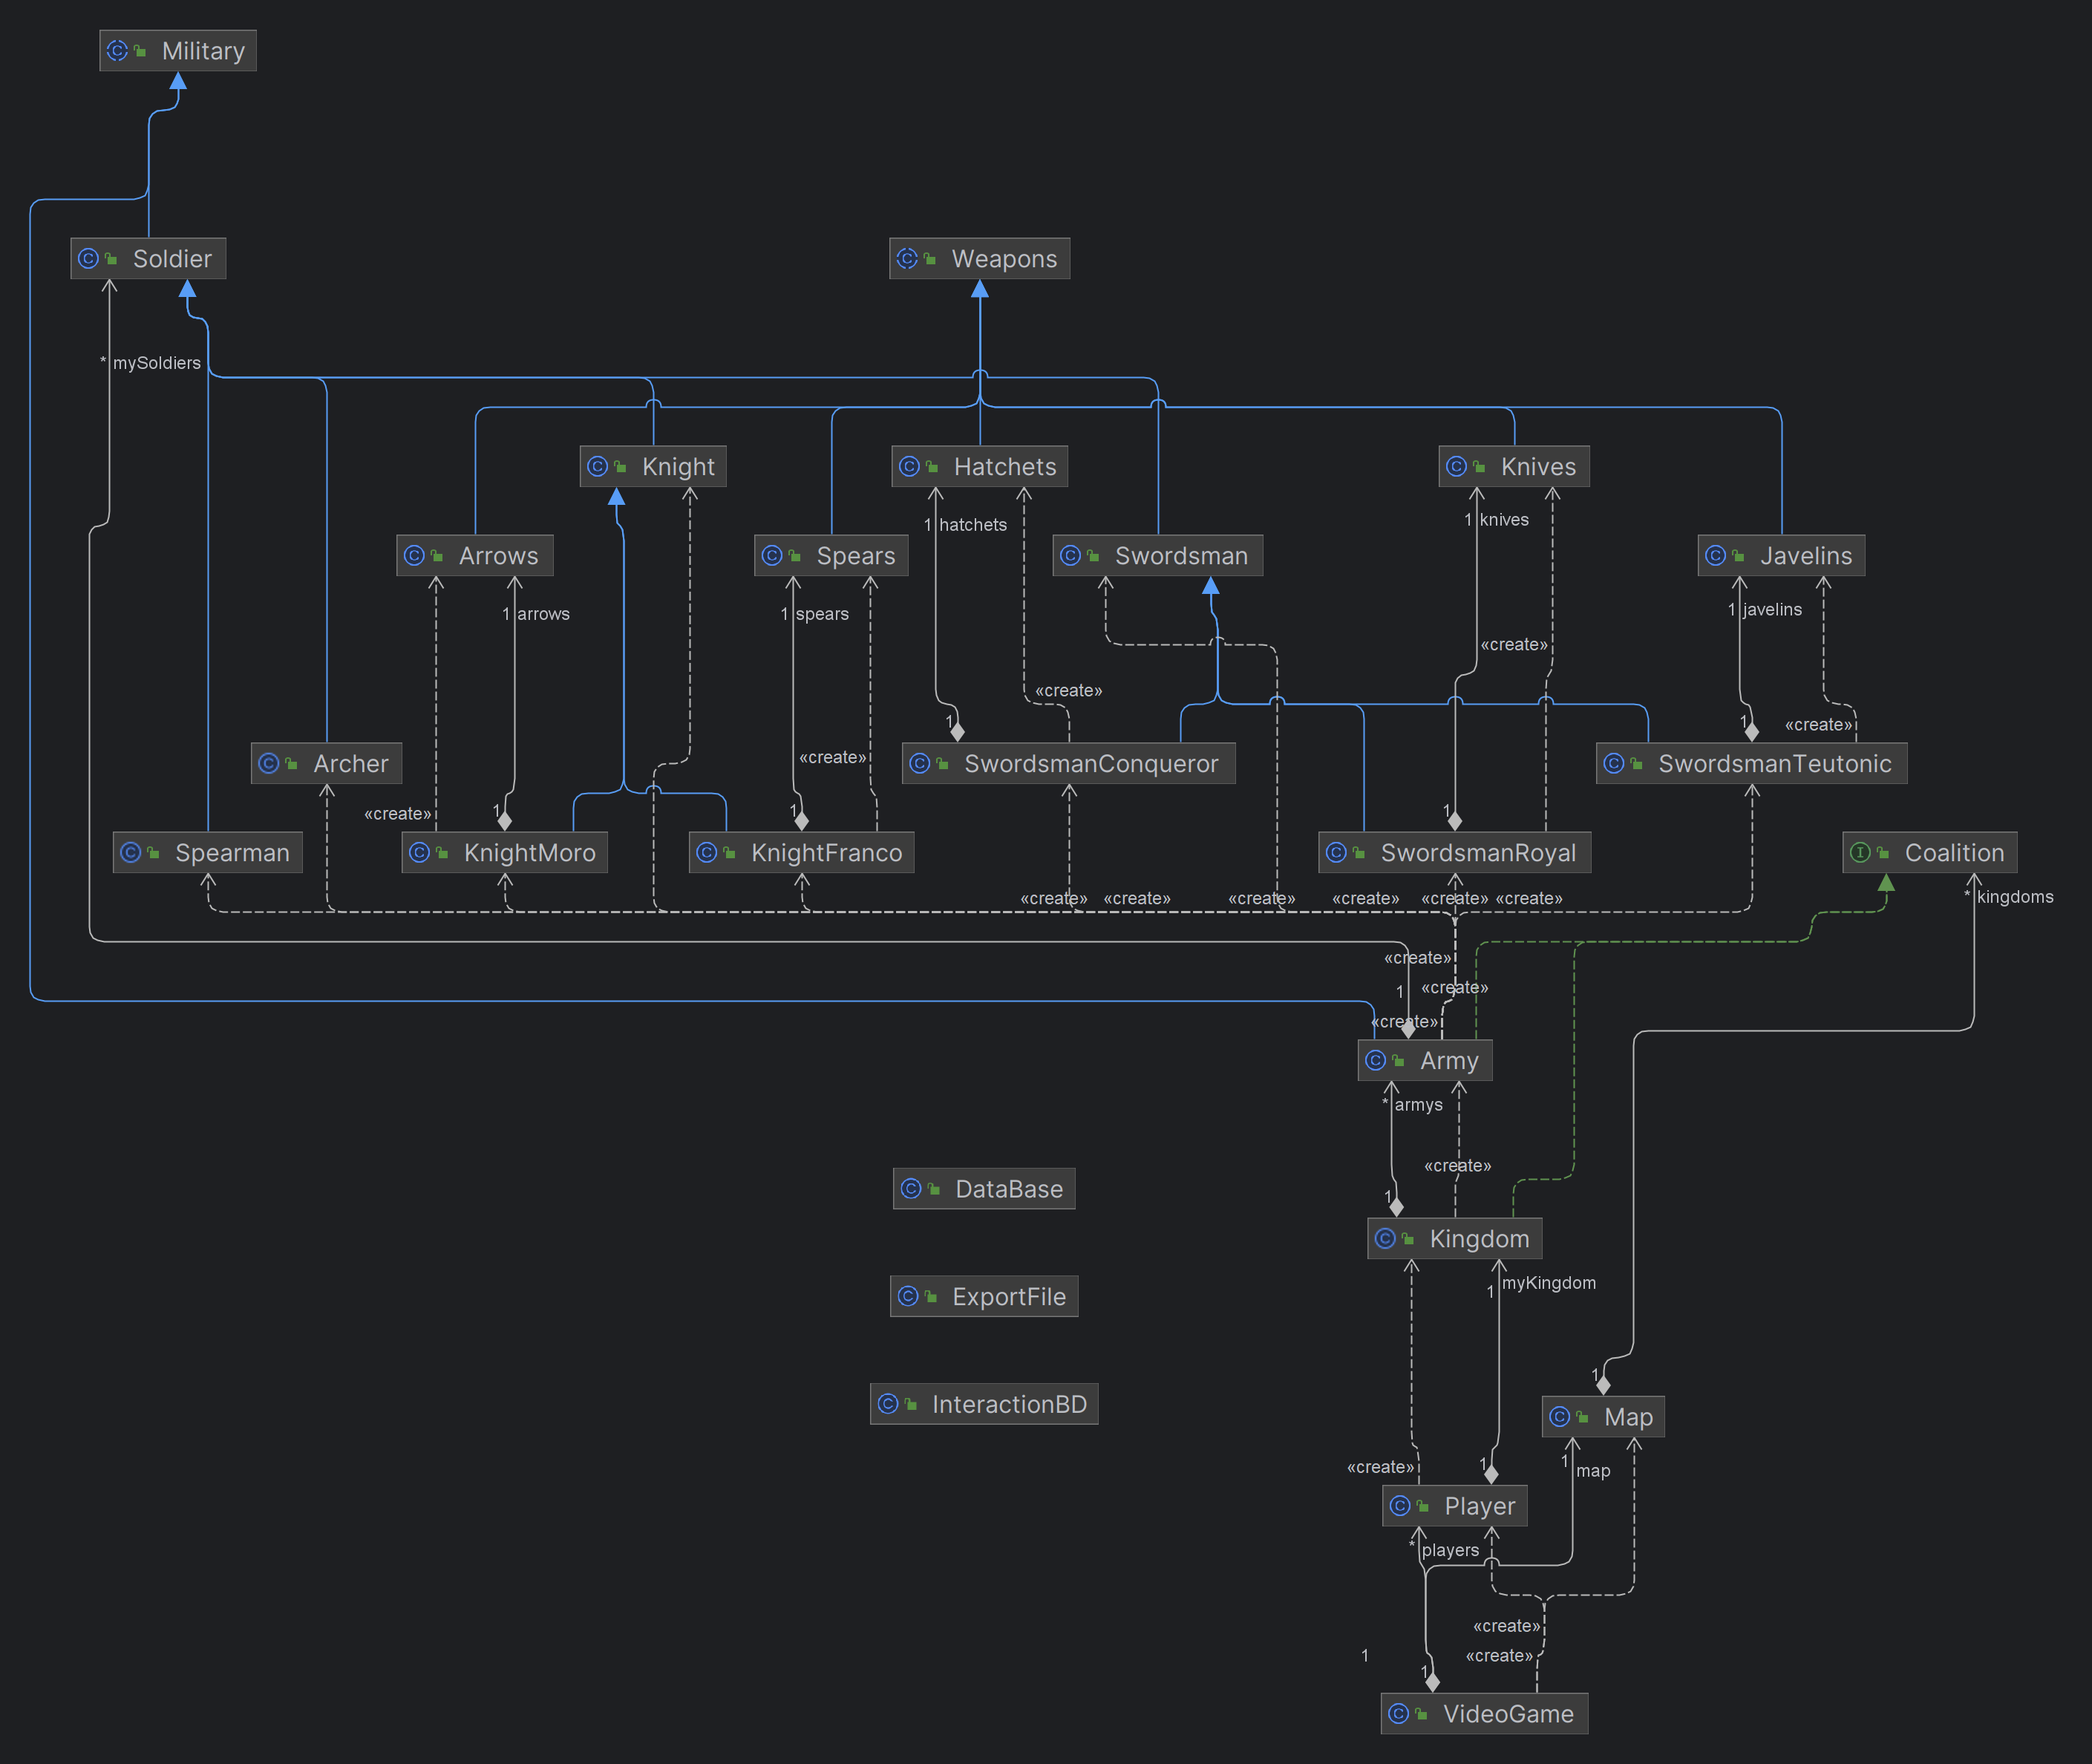
\includegraphics[width=0.9\textwidth,keepaspectratio]{img/DiagramaUML2.png}
        \caption{Relaciones de dependencia entre las clases}
    \end{figure}

%%%%%%%%%%%%%%%%%%%%

	\begin{itemize}
		\item Se puede apreciar la clase Soldier y todas sus subclases, ademas de las subclases de unidades especiales.
		\item Todas las clases de armas son subclases de la calse abstracta Weapons.java.
		\item Tambien se aprecia la composicion de la clase Soldier, con respecto a la clase Army. Asimismo, estas dos clases son subclases de la clase abstracta Military.java.
		\item De igual forma se aprecia la composicion de la clase Army, con respecto a la clase Kingdom. Asimismo, estas dos clases comparten la interface Coalition.java.
		\item Existe la clase Map que representa el tablero del VideoJuego.
            \item Se creo la clase DataBase.java con la estructura de diseño de singleton para tener una unica conexion definida hacia la base de datos.
            \item Tambien existe la clase InteractionBD.java a traves de la cual se realizan todas la consultas, imports, entre otros, hacia la base de datos.
		\item De igual forma, se presenta el archivo VideoGame.java que permitira la interaccion de todas las otras clases y el funcionamiento del VideoJuego.
	\end{itemize}

%%%%%%%%%%%%%%%%%%%%

	\subsection{Clases Utilizadas}
	
	\begin{itemize}
		\item Archer.java
            \item Army.java
            \item Arrows.java
            \item Coalition.java
            \item DataBase.java
            \item ExportFile.java
            \item Hatchets.java
            \item InteractionBD.java
            \item Javelins.java
            \item Kingdom.java
            \item Knight.java
            \item KnightFranco.java
            \item KnightMoro.java
            \item Knives.java
            \item Map.java
            \item Military.java
            \item Player.java
            \item Soldier.java
            \item Spearman.java
            \item Spears.java
            \item Swordsman.java
            \item SwordsmanConqueror.java
            \item SwordsmanRoyal.java
            \item SwordsmanTeutonic.java
            \item VideoGame.java
            \item Weapons.java
	\end{itemize}
	
%%%%%%%%%%%%%%%%%%%%%%%%%%%%%%%%%%%%%%%%%%%%%%%%%%%%%%%%%%%%%%%%%%%
%%%%%%%%%%%%%%%%%%%%%%%%%%%%%%%%%%%%%%%%%%%%%%%%%%%%%%%%%%%%%%%%%%%
%%%%%%%%%%%%%%%%%%%%%%%%%%%%%%%%%%%%%%%%%%%%%%%%%%%%%%%%%%%%%%%%%%%

    
\subsection{Interfaz Gráfica}
	
	\begin{figure}[H]
        \centering
		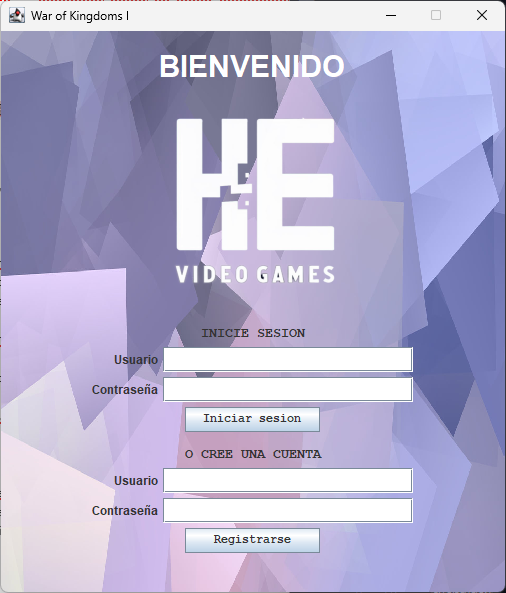
\includegraphics[width=0.6\textwidth,keepaspectratio]{img/Menu_Sesion.png}
        \caption{Menú de Sesion del VideoJuego}
    \end{figure}

        \begin{itemize}	
		\item Se crea una ventana principal (window0) con un tamaño específico, título, ubicación central, y diseño no redimensionable.
            \item Se establece una imagen de fondo en la ventana principal.
            \item Se añade un título "BIENVENIDO" y una imagen de login con un logo escalado al centro de la ventana.
            \item Se crean botones para iniciar sesión y registrarse, con un diseño específico y estilo de fuente.
            \item Se definen campos de texto para el nombre de usuario y contraseña, junto con etiquetas descriptivas.
            \item Se configuran acciones al presionar "Enter" en los campos de texto para simular un clic en el botón de inicio de sesión.
            \item Se organizan los elementos en paneles y se agregan a la ventana principal.
            \item Se manejan eventos de clic en los botones de inicio de sesión y registro, verificando la autenticación y registrando nuevos usuarios mediante interacción con una base de datos (InteractionBD).
            \item Si la autenticación o el registro son exitosos, se abre una ventana principal (mainWindow).
            \item La ventana principal se hace visible al final.
	\end{itemize}
    
    
    \begin{figure}[H]
        \centering
		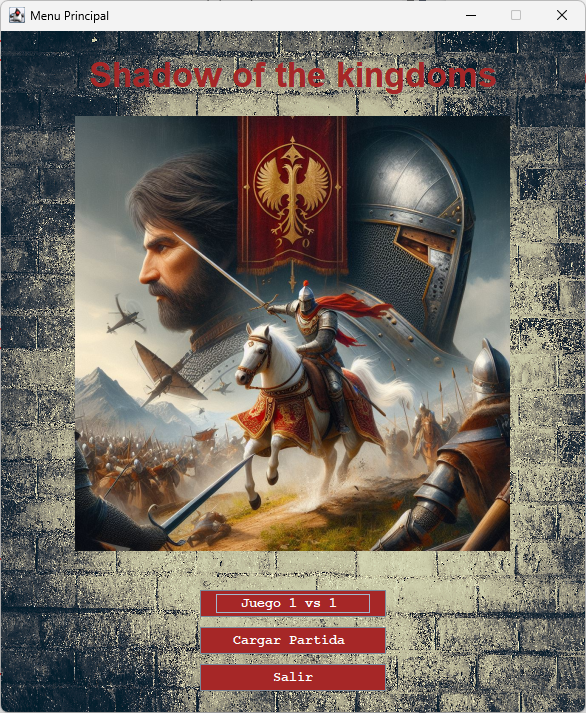
\includegraphics[width=0.8\textwidth,keepaspectratio]{img/Menu_Principal.png}
        \caption{Menú de Principal del VideoJuego}
    \end{figure}

    \begin{itemize}	
		\item El código cierra la ventana actual, crea y muestra una nueva ventana para el menú principal de un juego llamado "Shadow of the Kingdoms".
            \item La ventana contiene un título, una imagen de portada, y botones para opciones como iniciar un juego 1 vs 1, cargar una partida, o salir del juego.
            \item La interfaz gráfica utiliza colores y fuentes específicos para dar estilo a la presentación.
            \item El código también define acciones para los botones, como abrir una ventana de configuración de jugador al hacer clic en el primer botón, cargar una nueva partida al hacer clic en el segundo botón, y cerrar la aplicación al hacer clic en el tercer botón.
    \end{itemize}

    \begin{figure}[H]
        \centering
		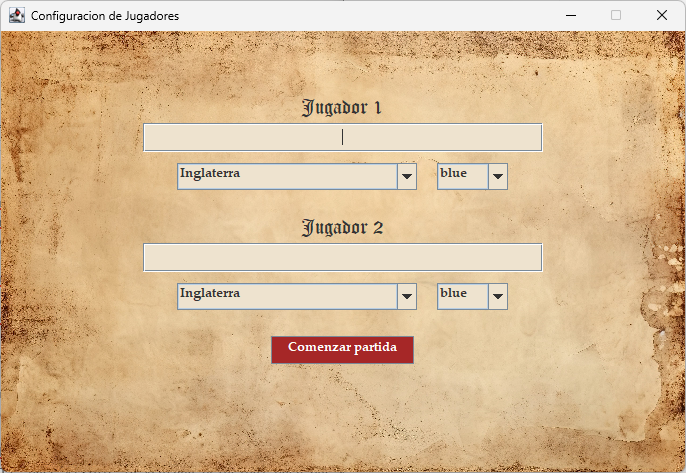
\includegraphics[width=0.75\textwidth,keepaspectratio]{img/Menu_Configuracion.png}
        \caption{Menú de Personalización del VideoJuego}
    \end{figure}

    \begin{itemize}	
		\item La función playerSetupWindow toma una ventana existente (window), la cierra y crea una nueva ventana para la configuración de jugadores.
            \item Se inicializa el mapa y una lista de jugadores.
            \item Se crean listas para almacenar componentes de la interfaz gráfica, como campos de texto y cuadros de selección.
            \item Se configura la apariencia básica de la nueva ventana, incluyendo una imagen de fondo.
            \item Se crea un panel principal vertical que contiene estructuras de ingreso para dos jugadores.
            \item Cada estructura de ingreso se crea mediante la función createPlayerPanel, que incluye un número de jugador, un campo de texto para el nombre, y cuadros de selección para el reino y el color.
            \item Se añade un botón "Comenzar partida" que recoge la información ingresada y crea objetos de jugador con esos datos. Luego, inicia el juego.
            \item La función createPlayerPanel retorna un panel con los elementos de entrada y selección para un jugador específico.
	\end{itemize}

    \begin{figure}[H]
        \centering
		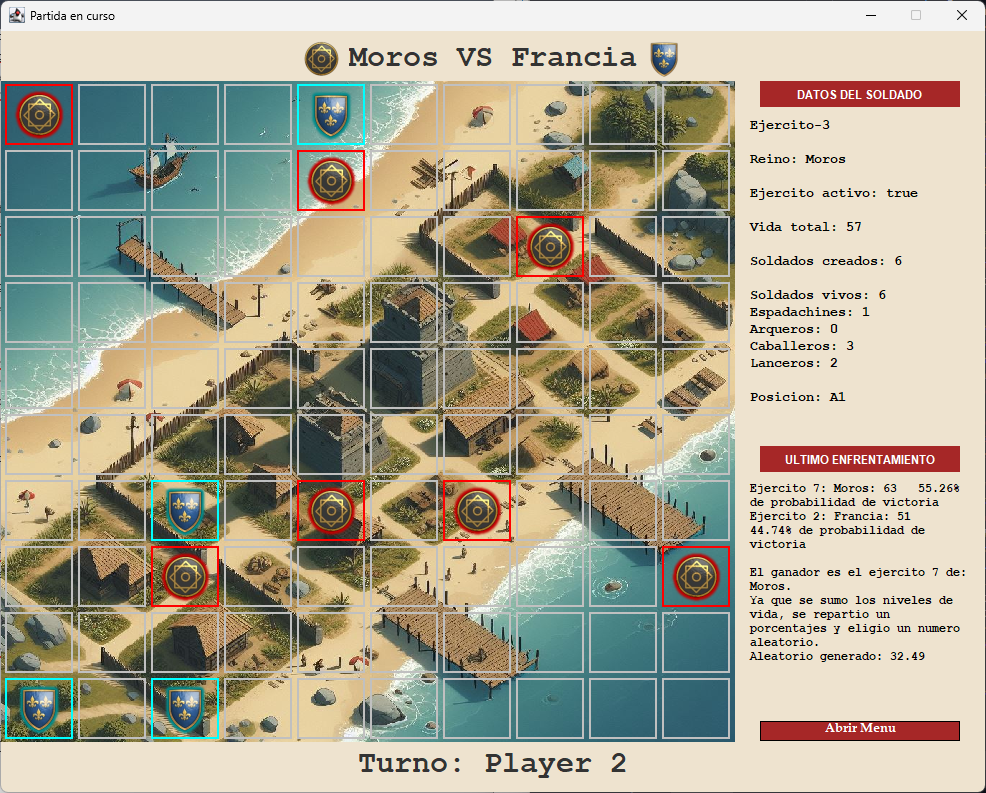
\includegraphics[width=0.9\textwidth,keepaspectratio]{img/Menu_Tablero_Ejercitos.png}
        \caption{Ventana del VideoJuego - Ejercitos}
    \end{figure}

    \begin{itemize}	
		\item La función startGame toma una ventana existente (window), la cierra y crea una nueva ventana para la partida en curso.
            \item Se configura la apariencia básica de la nueva ventana, incluyendo el tamaño, la ubicación, y la no redimensionabilidad.
            \item Se crea un encabezado que muestra los reinos en guerra (kingdom1 VS kingdom2) y las imágenes de los reinos.
            \item Se crea y muestra un mapa utilizando la función createMap y se añade a la ventana.
            \item Se crea un panel de información que muestra datos sobre los ejércitos y soldados.
            \item Se añaden paneles y etiquetas para mostrar información relevante, como datos del soldado y el resultado de la batalla.
            \item Se añade un botón "Abrir Menú" que llama a la función gameMenu al hacer clic.
            \item Se configura la parte inferior de la ventana para mostrar el turno actual del jugador.
            \item Se añade un listener para la tecla Escape, que llama a la función gameMenu al presionar Escape.
            \item La ventana se hace visible al final.
	\end{itemize}
    \begin{itemize}	
		\item Al llamar a la función createMap, se crea un panel (mapArmys) con un diseño de cuadrícula para representar el mapa de ejércitos.
            \item El mapa de ejércitos se inicializa con un nuevo objeto de mapa proporcionado como parámetro.
            \item Se llama al método createBoardArmys del objeto map para generar la configuración inicial del tablero de ejércitos.
            \item Este método utiliza información sobre los reinos de los jugadores para establecer la distribución inicial de los ejércitos en el tablero.
            \item Se configuran botones en el panel de ejércitos (mapArmys). Cada botón se asigna a un ActionListener llamando al método interaction al hacer clic, y se añade un MouseListener para llamar al método infoMilitary cuando el mouse entra en el área del botón.
            \item Los botones se añaden al panel de ejércitos, completando así la representación visual del mapa de ejércitos.
	\end{itemize}

\newpage
    \begin{figure}[H]
        \centering
		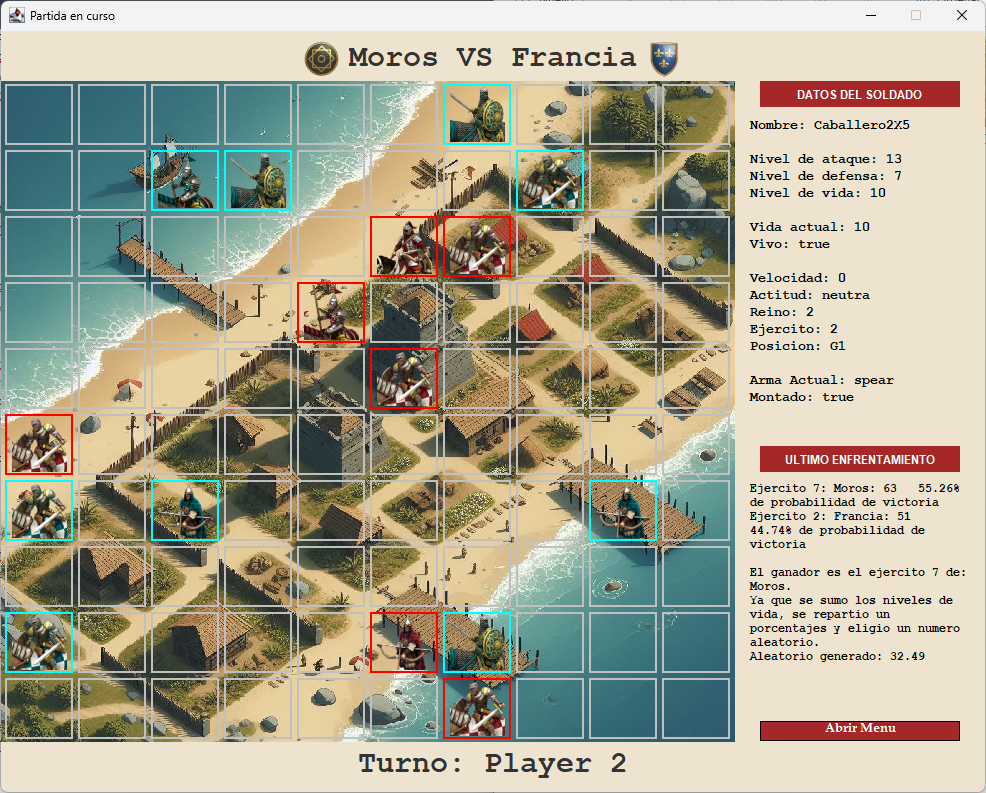
\includegraphics[width=0.9\textwidth,keepaspectratio]{img/Menu_Tablero_Soldados.png}
        \caption{Ventana del VideoJuego - Soldados}
    \end{figure}

    \begin{itemize}	
		\item Al enfrentarse 2 ejercitos, se llema a la función confrontation donde se crea un nuevo panel (mapSoldiers) con un diseño de cuadrícula para representar el mapa de soldados.
            \item El método createBoardSoldiers del objeto map se llama para configurar la distribución inicial de los soldados en el tablero, utilizando información sobre los ejércitos aliados y enemigos.
            \item Se establece la variable then como nula.
            \item Se configuran botones en el panel de soldados (mapSoldiers). Cada botón se asigna a un ActionListener llamando al método interaction al hacer clic, y se añade un MouseListener para llamar al método infoMilitary cuando el mouse entra en el área del botón.
            \item Los botones se añaden al panel de soldados.
            \item Se elimina cualquier componente existente en el panel de juego (mapSpace).
            \item El panel de soldados se añade al panel de juego.
            \item Se actualiza y repinta la ventana principal (window2) para reflejar los cambios, mostrando el tablero de los soldados.
	\end{itemize}


\newpage
    \begin{figure}[H]
        \centering
		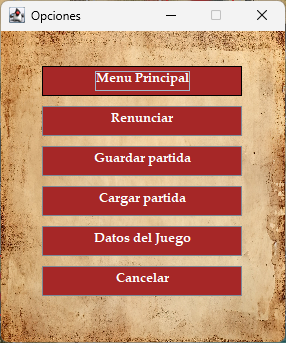
\includegraphics[width=0.45\textwidth,keepaspectratio]{img/Menu_Opciones.png}
        \caption{Menú de Pausa}
    \end{figure}

    \begin{itemize}	
            \item Se crea una nueva ventana (windowGameMenu) con configuraciones específicas de tamaño, cierre, ubicación y no redimensionamiento.
            \item Se establece una imagen de fondo en la ventana utilizando un panel ImagePanel.
            \item Se crea un panel (panel) para organizar los botones en forma de columna utilizando BoxLayout en el eje Y.
            \item Se crean varios botones para diferentes opciones del menú, cada uno con su acción correspondiente al hacer clic.
            \item Los botones se añaden al panel, separados por espacios rígidos para dar un formato adecuado.
            \item Se configuran las propiedades visuales de los botones, como el color del texto, el fondo y la fuente.
            \item Se añade un borde alrededor del panel para darle un aspecto estéticamente agradable.
            \item El panel se añade a la ventana en la región central.
            \item La ventana se hace visible al final.
	\end{itemize}



\newpage
    \begin{figure}[H]
        \centering
		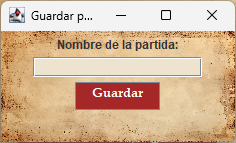
\includegraphics[width=0.45\textwidth,keepaspectratio]{img/Menu_Guardar_Partida.png}
        \caption{Menú de Guardar la partida}
    \end{figure}

    \begin{itemize}	
            \item Se crea una nueva ventana (windowSaveGame) con configuraciones específicas de tamaño, ubicación, cierre y diseño de flujo (FlowLayout).
            \item Se establece una imagen de fondo en la ventana utilizando un panel ImagePanel.
            \item Se crean componentes de interfaz de usuario, como una etiqueta (lblNombre) para indicar el propósito del campo de texto, un campo de texto (txtNombre) para ingresar el nombre de la partida, y un botón (btnGuardar) para realizar la acción de guardar.
            \item  Se configuran propiedades visuales, como el fondo y la fuente, para algunos de los componentes.
            \item Se añade un ActionListener al botón de guardar (btnGuardar).
            \item Cuando se presiona el botón, se obtiene el texto ingresado en el campo de texto y se utiliza para guardar la partida utilizando el método InteractionBD.saveGame(). Luego, la ventana de guardar se cierra.
            \item Los componentes se añaden a la ventana en el orden deseado.
            \item La ventana de guardar se hace visible al final.
	\end{itemize}

\newpage
    \begin{figure}[H]
        \centering
		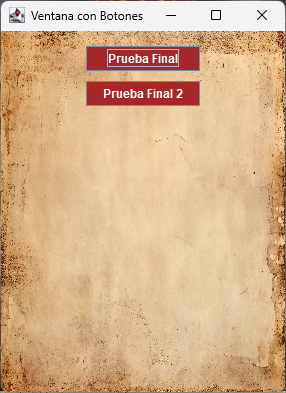
\includegraphics[width=0.45\textwidth,keepaspectratio]{img/Menu_Cargar_Partida.png}
        \caption{Menú de Cargar una partida}
    \end{figure}

    \begin{itemize}	
            \item Se crea una nueva ventana (windowLoadGame) con configuraciones específicas de tamaño, ubicación y cierre.
            \item Se establece una imagen de fondo en la ventana utilizando un panel ImagePanel.
            \item Se obtienen las etiquetas de las partidas guardadas desde la base de datos mediante el método InteractionBD.getAllSavedGames() y se almacenan en un ArrayList llamado etiquetas.
            \item Se crea un panel para organizar los botones en forma de columna, con un fondo transparente.
            \item Se crean botones para cada etiqueta obtenida. Cada botón tiene un fondo y un color de texto específicos. Además, se añade un ActionListener a cada botón.
            \item Cuando se presiona un botón, se utiliza la etiqueta asociada para cargar la partida correspondiente desde la base de datos mediante InteractionBD.loadGame(etiqueta). Se verifica la integridad de los datos cargados y se actualizan las variables globales players y map.
            \item Se añaden los botones al panel y se establece un espacio entre ellos.
            \item Se configura un borde con espacio alrededor del panel.
            \item Se agrega el panel a la ventana en el centro.
            \item Finalmente, la ventana de carga se hace visible.
	\end{itemize}

\newpage
     \begin{figure}[H]
        \centering
		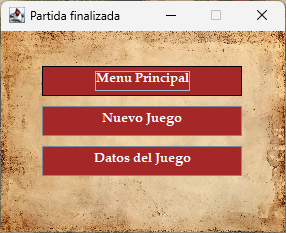
\includegraphics[width=0.45\textwidth,keepaspectratio]{img/Menu_Fin_Partida.png}
        \caption{Menú al finalizar partida}
    \end{figure}

    \begin{itemize}	
            \item Se crea una nueva ventana (finishWindow) con configuraciones específicas de tamaño, ubicación y cierre.
            \item Se establece una imagen de fondo en la ventana utilizando un panel ImagePanel.
            \item Se crea un panel para organizar los botones en forma de columna, con un fondo transparente y una dimensión preferida.
            \item Se crean botones con etiquetas específicas y configuraciones de estilo. Cada botón tiene un ActionListener asociado.
            \item El primer botón ("Menu Principal") permite regresar al menú principal, cerrando la ventana actual y mostrando el menú principal.
            \item El segundo botón ("Nuevo Juego") cierra la ventana actual y muestra la ventana de configuración de jugadores para iniciar un nuevo juego.
            \item El tercer botón ("Datos del Juego") ejecuta una acción para exportar los datos del juego a un archivo de texto mediante ExportFile.fileWriter(players, map).
            \item Se añade espacio entre los botones y en los bordes del panel.
            \item El panel se agrega a la ventana en el centro.
            \item Finalmente, la ventana emergente se hace visible.
	\end{itemize}
	

\newpage






%%%%%%%%%%%%%%%%%%%%%%%%%%%%%%%%%%%%%%%%%%%%%%%%%

\subsection{Base de Datos}

	\lstinputlisting[language=Java, firstline=1, lastline=50, firstnumber=1, caption={Conexion a Base de Datos con Singleton},numbers=left,]{src/DataBase.java}

        \begin{itemize}	
            \item Se declara una variable estática instance de tipo DataBase para almacenar la única instancia de la clase.
            \item La clase tiene un campo privado connection que representa la conexión a la base de datos.
            \item Se definen constantes JDBC-URL, USER y PASSWORD que contienen la URL de conexión JDBC, el usuario y la contraseña para acceder a la base de datos.
            \item El constructor privado de la clase carga el driver de JDBC y establece la conexión a la base de datos usando las credenciales proporcionadas.
            \item Se implementa un método estático getInstance que devuelve la única instancia de la clase DataBase, creándola si aún no existe.
            \item Se proporciona un método getConnection que devuelve la conexión a la base de datos.
            \item El uso del patrón Singleton asegura que solo haya una instancia de la clase DataBase y proporciona un punto de acceso global a la conexión de la base de datos en toda la aplicación.
	\end{itemize}
    

    \lstinputlisting[language=Java, firstline=22, lastline=63, firstnumber=22, caption={Guardar Partida},numbers=left,]{src/InteractionBD.java}

        \begin{itemize}	
            \item La clase tiene un campo estático fileName que representa el nombre fijo del archivo en el cual se guarda la partida (saveGame.txt).
            \item El método público saveGame recibe el nombre de la partida (gameName) y un arreglo de objetos (game). Utiliza un ObjectOutputStream para escribir el arreglo de objetos en el archivo mencionado. Luego, llama al método privado saveFileToDatabase para guardar el archivo en la base de datos.
            \item El método privado saveFileToDatabase realiza las siguientes acciones:
            \begin{itemize}	
                \item Establece una conexión a la base de datos utilizando la clase DataBase.
                \item Define una consulta SQL para insertar el nombre de la partida y el contenido del archivo en la tabla savegame.
                \item Utiliza un PreparedStatement para ejecutar la consulta, asignando el nombre de la partida y el contenido del archivo al statement.
                \item Lee el contenido del archivo como un array de bytes y lo almacena en la base de datos como un campo binario (BLOB).
                \item Ejecuta la consulta SQL para guardar el archivo en la base de datos.
            \end{itemize}
	\end{itemize}

    \lstinputlisting[language=Java, firstline=65, lastline=119, firstnumber=65, caption={Cargar Partida},numbers=left,]{src/InteractionBD.java}

        \begin{itemize}	
            \item getAllSavedGames:
            \begin{itemize}	
                \item Este método obtiene todos los nombres de las partidas guardadas en la base de datos.
                \item Realiza una consulta SQL para seleccionar los nombres de las partidas (SELECT game_name FROM savegame).
                \item Itera sobre el resultado de la consulta y agrega cada nombre de partida a un ArrayList llamado gameNames.
                \item Retorna el ArrayList que contiene los nombres de todas las partidas guardadas.
            \end{itemize}
            \item loadGame:
            \begin{itemize}	
                \item Este método carga una partida desde la base de datos según el nombre de la partida proporcionado.
                \item Realiza una consulta SQL para seleccionar el contenido de la partida (SELECT file_game FROM savegame WHERE game_name = ?).
                \item Utiliza un PreparedStatement para establecer el nombre de la partida en la consulta.
                \item Lee el resultado de la consulta, que contiene el contenido de la partida como un flujo de bytes.
                \item Deserializa el objeto desde el flujo de bytes utilizando un ObjectInputStream para obtener el arreglo de objetos (Object[]).
                \item Retorna el arreglo de objetos que representa la partida cargada.
            \end{itemize}
	\end{itemize}

    \lstinputlisting[language=Java, firstline=121, lastline=202, firstnumber=121, caption={Ingresar y Registrar Usuario},numbers=left,]{src/InteractionBD.java}

        \begin{itemize}	
            \item authenticateUser:
            \begin{itemize}	
                \item Este método verifica si un usuario está registrado en el sistema.
                \item Utiliza una consulta SQL para seleccionar filas de la tabla "users" que coincidan con el nick\_name y la contraseña proporcionados.
                \item Retorna true si al menos una fila es devuelta por la consulta, indicando que el usuario está registrado; de lo contrario, retorna false.
                \item Maneja excepciones de SQL, imprimiendo la traza de la excepción en caso de error.
            \end{itemize}
            \item registerUser:
            \begin{itemize}
                \item Este método registra un nuevo usuario en el sistema.
                \item Verifica primero si ya existe un usuario con el mismo nick\_name utilizando el método userExists.
                \item Si el usuario no existe, procede a realizar una consulta de inserción SQL para agregar un nuevo usuario a la tabla "users".
                \item Retorna true si al menos una fila fue afectada por la inserción, indicando que el registro fue exitoso; de lo contrario, retorna false.
                \item Maneja excepciones de SQL, imprimiendo la traza de la excepción en caso de error.
            \end{itemize}
            \item userExists:
            \begin{itemize}
                \item Este método es un auxiliar utilizado por registerUser para verificar si ya existe un usuario con el mismo nick\_name.
                \item Utiliza una consulta SQL para seleccionar filas de la tabla "users" que coincidan con el nick\_name proporcionado.
                \item Retorna true si al menos una fila es devuelta por la consulta, indicando que el usuario ya existe; de lo contrario, retorna false.
                \item Maneja excepciones de SQL, imprimiendo la traza de la excepción en caso de error.
            \end{itemize}
	\end{itemize}

 %%%%%%%%%%%%%%%%%%%%%%%%%%%%%%%%%%%%%%%%%%%%%%%%%

\subsection{Exportar datos del VideoJuego}

	\lstinputlisting[language=Java, firstline=1, lastline=50, firstnumber=1, caption={Exportar Archivo con Datos del VideoJuego},numbers=left,]{src/DataBase.java}

        \begin{itemize}	
            \item La función fileWriter recibe un ArrayList de jugadores (game) y un objeto Mapa (map) que representan el estado de una partida del juego "Shadow of the Kingdoms".
            \item Crea un archivo de texto con el nombre "DataGame.txt" y utiliza un objeto PrintWriter para escribir en él.
            \item Imprime información sobre la partida, incluyendo los nombres de los reinos que participan, los ejercitos de cada reino, los soldados de cada ejercito y detalles del mapa.
            \item Itera sobre los jugadores en el ArrayList y escribe información sobre cada uno, incluyendo detalles sobre su reino (MyKingdom) utilizando el método dataFile() del reino.
            \item Cierra el objeto PrintWriter después de completar la escritura en el archivo.
            \item Imprime un mensaje en la consola indicando que la escritura en el archivo fue exitosa.
            \item Utiliza la clase Desktop para abrir el archivo recién creado con la aplicación predeterminada para archivos en el sistema.
            \item Maneja excepciones de IO, imprimiendo mensajes de error en caso de problemas al escribir o abrir el archivo.
	\end{itemize}

        \begin{lstlisting}[language=bash,caption={Ejemplo de los datos del VideoJuego guardados}][H]
                Shadow of the kingdoms

                Inglaterra VS Francia


    Mapa: Territorio: campo abierto	Cantidad de ejercitos: 7


    Player 1: NickName: 	 Reino: Inglaterra	 Color: red


    Reino: Inglaterra

    Ejercito: Ejercito-1	 Activo: true	 Vida total: 38	 Soldados creados: 4	 Soldados vivos: 4	 Espadachines: 2	 Arqueros: 0	 Caballeros: 1	 Lanceros: 1	 Posicion: A5

    Soldado: Espadachin_Real	 Nivel de ataque: 10	 Nivel de defensa: 8	 Nivel de vida: 12	 Vida actual: 12	 Velocidad: 0	 Actitud: neutra	 Vivo: true	 Reino: 1	 Ejercito: 1	 Posicion: ...
	\end{lstlisting}
	
	\begin{itemize}
		\item En el archivo creado se muestra un resumen de todo los datos del VideoJuego, describiendo todos los atributos de los Players, de sus Reinos, Ejercitos y Soldados.
	\end{itemize}
 

%%%%%%%%%%%%%%%%%%%%%%%%%%%%%%%%%%%%%%%%%%%%%%%%%%%%%%%%%%%%%%%%%%%
	
	\begin{lstlisting}[language=bash,caption={Commits del archivo VideoGame.java}][H]
		$ git commit -m "Clase VideoGame"
		$ git commit -m "Clase ExportFile"
		$ git commit -m "Clase DataBase"
		$ git commit -m "Clase Interaction BD"  
		$ git commit -m "Imagenes"
		$ git commit -m "Librerias"
		$ git commit -m "VideoGame.jar"
	\end{lstlisting}
	
	\begin{itemize}
		\item Estos son los commits más importantes realizados durante la creación de VideoGame.java, puesto que los métodos que se registrán, resultan ser los determinantes para el funcionamiento y estructura grafica principal de programa.
		\item Código del commit 1: 1e52bd271e5046b38f4117f18c3fe504a0991c03
		\item Código del commit 2: e36bec829e2cb039555d4edecf2ada035b070677
		\item Código del commit 3: f1597abeff86b1596bc5d8c149455034bf9e4ec3
		\item Código del commit 4: cfd6b30795d3b294d9819be57ee0f16d1ec4e8a2
		\item Código del commit 5: 7d9356acb9ff666151f9ba94ce7c29d868d3ffe2
		\item Código del commit 6: 20b3374f9a992c8feb61dead9502dc68f77f09e2
		\item Código del commit 7: 3cc881520dbbca53c54e86dc303ce184df91a763
        
	\end{itemize}
	
%%%%%%%%%%%%%%%%%%%%%%%%%%%%%%%%%%%%%%%%%%%%%%%%%%%%%%%%%%%%%%%%%%%

\newpage
	\subsection{Estructura de laboratorio Final}
	\begin{itemize}	
		\item El contenido que se entrega en este laboratorio es el siguiente:
	\end{itemize}
	
\begin{lstlisting}[style=ascii-tree]
    labFinal/
    
    |--- Archer.class
    |--- Archer.java
    |--- Army.class
    |--- Army.java
    |--- Arrows.class
    |--- Arrows.java
    |--- Coalition.class
    |--- Coalition.java
    |--- DataBase.class
    |--- DataBase.java
    |--- DataGame.txt
    |--- ExportFile.class
    |--- ExportFile.java
    |--- Hatchets.class
    |--- Hatchets.java
    |--- InteractionBD.class
    |--- InteractionBD.java
    |--- Javelins.class
    |--- Javelins.java
    |--- Kingdom.class
    |--- Kingdom.java
    |--- Knight.class
    |--- Knight.java
    |--- KnightFranco.class
    |--- KnightFranco.java
    |--- KnightMoro.class
    |--- KnightMoro.java
    |--- Knives.class
    |--- Knives.java
    |--- MANIFEST.MF
    |--- Map$1.class
    |--- Map$2.class
    |--- Map.class
    |--- Map.java
    |--- Military.class
    |--- Military.java
    |--- Player.class
    |--- Player.java
    |--- saveGame.txt
    |--- Soldier.class
    |--- Soldier.java
    |--- Spearman.class
    |--- Spearman.java
    |--- Spears.class
    |--- Spears.java
    |--- Swordsman.class
    |--- Swordsman.java
    |--- SwordsmanConqueror.class
    |--- SwordsmanConqueror.java
    |--- SwordsmanRoyal.class
    |--- SwordsmanRoyal.java
    |--- SwordsmanTeutonic.class
    |--- SwordsmanTeutonic.java
    |--- VideoGame$1.class
    |--- VideoGame$2.class
    |--- VideoGame$3.class
    |--- VideoGame$4.class
    |--- VideoGame$5.class
    |--- VideoGame$6.class
    |--- VideoGame$ImagePanel.class
    |--- VideoGame.class
    |--- VideoGame.jar
    |--- VideoGame.java
    |--- Weapons.class
    |--- Weapons.java
    |--- lib
        |--- mysql-connector-j-8.3.0.jar
    |--- src
        |--- ...
        |--- swordsman_yellow.png

\end{lstlisting}    

	\section{\textcolor{red}{Rúbricas}}
	
	\subsection{\textcolor{red}{Entregable Informe}}
	\begin{table}[H]
		\caption{Tipo de Informe}
		\setlength{\tabcolsep}{0.5em} % for the horizontal padding
		{\renewcommand{\arraystretch}{1.5}% for the vertical padding
		\begin{tabular}{|p{3cm}|p{12cm}|}
			\hline
			\multicolumn{2}{|c|}{\textbf{\textcolor{red}{Informe}}}  \\
			\hline 
			\textbf{\textcolor{red}{Latex}} & \textcolor{blue}{El informe está en formato PDF desde Latex,  con un formato limpio (buena presentación) y facil de leer.}   \\ 
			\hline 
			
			
		\end{tabular}
	}
	\end{table}
	
	\clearpage
	
	\subsection{\textcolor{red}{Rúbrica para el contenido del Informe y demostración}}
	\begin{itemize}			
		\item El alumno debe marcar o dejar en blanco en celdas de la columna \textbf{Checklist} si cumplio con el ítem correspondiente.
		\item Si un alumno supera la fecha de entrega,  su calificación será sobre la nota mínima aprobada, siempre y cuando cumpla con todos lo items.
		\item El alumno debe autocalificarse en la columna \textbf{Estudiante} de acuerdo a la siguiente tabla:
	
		\begin{table}[ht]
			\caption{Niveles de desempeño}
			\begin{center}
			\begin{tabular}{ccccc}
    			\hline
    			 & \multicolumn{4}{c}{Nivel}\\
    			\cline{1-5}
    			\textbf{Puntos} & Insatisfactorio 25\%& En Proceso 50\% & Satisfactorio 75\% & Sobresaliente 100\%\\
    			\textbf{2.0}&0.5&1.0&1.5&2.0\\
    			\textbf{4.0}&1.0&2.0&3.0&4.0\\
    		\hline
			\end{tabular}
		\end{center}
	\end{table}	
	
	\end{itemize}
	
	\begin{table}[H]
		\caption{Rúbrica para contenido del Informe y demostración}
		\setlength{\tabcolsep}{0.5em} % for the horizontal padding
		{\renewcommand{\arraystretch}{1.5}% for the vertical padding
		%\begin{center}
		\begin{tabular}{|p{2.7cm}|p{7cm}|x{1.3cm}|p{1.2cm}|p{1.5cm}|p{1.1cm}|}
			\hline
    		\multicolumn{2}{|c|}{Contenido y demostración} & Puntos & Checklist & Estudiante & Profesor\\
			\hline
			\textbf{1. GitHub} & Hay enlace URL activo del directorio para el  laboratorio hacia su repositorio GitHub con código fuente terminado y fácil de revisar. &2 &X &2 & \\ 
			\hline
			\textbf{2. Commits} &  Hay capturas de pantalla de los commits más importantes con sus explicaciones detalladas. (El profesor puede preguntar para refrendar calificación). &4 &X &4 & \\ 
			\hline 
			\textbf{3. Código fuente} &  Hay porciones de código fuente importantes con numeración y explicaciones detalladas de sus funciones. &2 &X &2 & \\ 
			\hline 
			\textbf{4. Ejecución} & Se incluyen ejecuciones/pruebas del código fuente  explicadas gradualmente. &2 &X &2 & \\ 
			\hline			
			\textbf{5. Pregunta} & Se responde con completitud a la pregunta formulada en la tarea.  (El profesor puede preguntar para refrendar calificación).  &2 &X &2 & \\ 
			\hline	
			\textbf{6. Fechas} & Las fechas de modificación del código fuente estan dentro de los plazos de fecha de entrega establecidos. &2 &X &2 & \\ 
			\hline 
			\textbf{7. Ortografía} & El documento no muestra errores ortográficos. &2 &X &2 & \\ 
			\hline 
			\textbf{8. Madurez} & El Informe muestra de manera general una evolución de la madurez del código fuente,  explicaciones puntuales pero precisas y un acabado impecable.   (El profesor puede preguntar para refrendar calificación).  &4 &X &4 & \\ 
			\hline
			\multicolumn{2}{|c|}{\textbf{Total}} &20 & &20 & \\ 
			\hline
		\end{tabular}
		%\end{center}
		%\label{tab:multicol}
		}
	\end{table}
	
\clearpage

\section{Referencias}
    \item \url{https://docs.oracle.com/javase/tutorial/java/IandI/polymorphism.html}
    \item \url{https://docs.oracle.com/javase/tutorial/java/IandI/subclasses.html}
    \item \url{https://docs.oracle.com/javase/tutorial/java/IandI/createinterface.html}
    \item \url{https://developer.oracle.com/es/learn/java-and-databases.html}
    \item \url{https://docs.oracle.com/javase/8/docs/api/java/io/File.html}
	
%\clearpage
%\bibliographystyle{apalike}
%\bibliographystyle{IEEEtranN}
%\bibliography{bibliography}
			
\end{document}